\section{Estudio de alternativas}\label{sec:estudio}
En este apartado se explorarán las diferentes alternativas disponibles para el
diseño del sistema. Se analizarán las características, ventajas y desventajas de
cada opción, con el objetivo de proporcionar una visión clara y fundamentada que
permita seleccionar la alternativa más adecuada para el proyecto. Las áreas de
estudio incluirán tanto el despliegue de infraestructura como otros aspectos
críticos del diseño del sistema, asegurando una evaluación integral y detallada
de las posibles soluciones.

Los criterios de evaluación en líneas generales son los ya vistos en la sección
\fullref{sec:alternativas}, es decir: \textbf{coste}, \textbf{complejidad},
\textbf{rendimiento y escalabilidad} y \textbf{licencias} (o, más bien, la
ausencia de ellas).

En esta sección se estudiarán las alternativas referentes a:

\begin{itemize}
	\item \textbf{\nameref{subsec:alt_despliegue}}
	\item \textbf{\nameref{subsec:alt_ingesta}}
	\item \textbf{\nameref{subsec:alt_proveedor}}
	\item \textbf{\nameref{subsec:alt_servicios}}
	\item \textbf{\nameref{subsec:alt_maquinas}}
\end{itemize}

El orden de estudio de las alternativas no es casual, sino que sigue un orden
lógico \textit{top-down} en el desarrollo del proyecto, comenzando por la
herramienta de despliegue y los componentes para centrarse posteriormente en
proveedores, servicios, etc.


\newpage{}
\subsection{Despliegue de infraestructura}\label{subsec:alt_despliegue}
A la hora de desplegar la infraestructura de un proyecto, se consideran varias
herramientas populares que permiten automatizar este proceso. Para este
proyecto, se analizarán algunas de las más extendidas: \textit{Terraform},
\textit{AWS CloudFormation} y \textit{Ansible}.


\subparagraph{Terraform} es una herramienta de código abierto desarrollada por
\textit{HashiCorp} que permite definir y desplegar infraestructura de forma
declarativa. \textit{Terraform} permite definir la infraestructura en un archivo
de configuración HCL, que describe los recursos que se desean crear y sus
dependencias. A partir de este archivo, \textit{Terraform} se encarga de
desplegar los recursos en el proveedor de nube especificado, que en el caso de
este proyecto es \textit{AWS}.

\begin{figure}[H]
	\centering
	
\includegraphics[width=0.2\textwidth]{logos/terraform.png}
	\caption{Logo de Terraform~\textregistered}
	\label{fig:terraform}
\end{figure}

\subparagraph{AWS CloudFormation} es un servicio de \textit{Amazon Web Services}
similar a \textit{Terraform} que permite definir y desplegar infraestructura en
la nube de forma declarativa. \textit{AWS CloudFormation} permite definir la
infraestructura o bien mediante un archivo de configuración (en formato JSON o
YAML), o bien gráficamente mediante diagramas, un punto muy fuerte a favor de
esta alternativa.

\begin{figure}[H]
	\centering
	
\includegraphics[width=0.2\textwidth]{logos/cloudformation.png}
	\caption{Logo de AWS CloudFormation~\textregistered}
	\label{fig:cloudformation}
\end{figure}

\subparagraph{Ansible} es una herramienta multi-propósito de automatización de tareas
entre las que se incluye el despliegue y orquestación de infraestructura. Se
trata de una herramienta desarrollada por \textit{Red Hat} que permite definir
la infraestructura mediante \textit{playbooks} escritos en YAML, que describen
las tareas a realizar y los servidores en los que se deben ejecutar.

\begin{figure}[H]
	\centering
	
\includegraphics[width=0.2\textwidth]{logos/ansible.png}
	\caption{Logo de Ansible~\textregistered}
	\label{fig:ansible}
\end{figure}

\paragraph{Comparación}
Comenzando la comparativa por la facilidad de uso de cada herramienta,
\textit{Terraform} es la alternativa planteada más fácil de usar, ya que permite
definir la infraestructura en un archivo con sintaxis sencilla y desplegarla con
un solo comando. Por otro lado, \textit{AWS CloudFormation} es un poco más
complejo de usar, ya que requiere definir la infraestructura en un archivo de
configuración o en un diagrama, y luego desplegarla mediante la consola de
\textit{AWS}. \textit{Ansible} es más complejo, ya que requiere definir
la infraestructura mediante \textit{playbooks} y ejecutarlos en los servidores,
pero es más flexible y potente que las otras dos herramientas.

Mientras que \textit{Terraform} y \textit{Ansible} son herramientas
\textit{multi-cloud}, lo que significa que funcionan con cualquier proveedor de
nube, \textit{AWS CloudFormation} es una herramienta específica de \textit{AWS}
y solo funciona con sus servicios.

Como punto importante, Terraform es la única herramienta de las tres con la que
se tiene experiencia previa dentro de la empresa, lo que facilitaría su
adopción y uso en el proyecto.

\paragraph{Decisión}
Ninguna de las alternativas consideradas es funcionalmente superior a las demás,
y se tratan de herramientas con características similares y una gran popularidad
en la industria. \textit{Sin embargo}, se decide utilizar \textit{Terraform}
para el despliegue de la infraestructura de este proyecto, ya que es la
herramienta más ``sencilla'', la que mejor se podría adaptar a las necesidades
del proyecto y la única que ya se ha usado en proyectos anteriores dentro de la
empresa.


\newpage{}
\subsection{Ingesta de datos}\label{subsec:alt_ingesta}
A partir del conjunto de tecnologías seleccionadas en la descripción detallada
del proyecto, se consdieran diversas tecnologías, como \textit{Redpanda},
\textit{AWS Glue} y \textit{Kafka} que permitan la ingesta datos de todas las
fuentes que requieren ser procesadas.


\subparagraph{Kafka} es una plataforma de transmisión de datos distribuida y de
código abierto que se utiliza para construir pipelines de datos en tiempo real y
aplicaciones de streaming. Desarrollada originalmente por LinkedIn y
posteriormente integrada en la Apache Software Foundation, \textit{Kafka} se ha
convertido en una de las tecnologías más populares para la gestión de flujos de
datos en tiempo real.

\begin{figure}[H]
	\centering
	
\includegraphics[width=0.2\textwidth]{logos/kafka.png}
	\caption{Logo de Kafka~\textregistered}
	\label{fig:kafka}
\end{figure}

Una de las principales ventajas de \textit{Kafka} es su capacidad para manejar
grandes volúmenes de datos con alta eficiencia y baja latencia. \textit{Kafka}
utiliza un modelo de publicación-suscripción, donde los productores publican
mensajes en temas y los consumidores se suscriben a estos temas para recibir
los mensajes. Esta arquitectura permite una alta escalabilidad y flexibilidad
en la gestión de datos.

A pesar de sus numerosas ventajas, \textit{Kafka} también presenta algunos
desafíos. La configuración y gestión de un clúster de \textit{Kafka} puede ser
compleja, especialmente en entornos de producción a gran escala. Además,
\textit{Kafka} depende de \textit{Zookeeper} para la coordinación, lo que añade
una capa adicional de complejidad en la administración del sistema.

En resumen, \textit{Kafka} es una solución robusta y escalable para la
transmisión de datos en tiempo real, ideal para aplicaciones que requieren alta
disponibilidad y procesamiento eficiente de grandes volúmenes de datos. Sin
embargo, su implementación y gestión requieren un conocimiento profundo de su
arquitectura y componentes.

\newpage{}
\subparagraph{Redpanda} es una plataforma de transmisión de datos en tiempo real
que se destaca por su alto rendimiento y baja latencia. Diseñada como una
alternativa moderna a \textit{Kafka}, \textit{Redpanda} ofrece una arquitectura
simplificada que elimina la necesidad de dependencias externas como
\textit{Zookeeper}. Esto no solo reduce la complejidad operativa, sino que
también mejora la eficiencia y la escalabilidad del sistema. \textit{Redpanda}
es compatible con la API de \textit{Kafka}, lo que facilita la migración de
aplicaciones existentes sin necesidad de cambios significativos en el código.
Además, su diseño optimizado para hardware moderno permite un procesamiento más
rápido y un uso más eficiente de los recursos, lo que la convierte en una opción
ideal para aplicaciones que requieren una transmisión de datos rápida y
confiable.

Sin embargo, \textit{Redpanda} también presenta algunos puntos en contra. Al ser
una tecnología relativamente nueva, su ecosistema y comunidad de usuarios no son
tan amplios como los de \textit{Kafka}, lo que puede limitar el acceso a
recursos y soporte. Además, aunque la compatibilidad con la API de
\textit{Kafka} es una ventaja, puede haber ciertas características y extensiones
específicas de \textit{Kafka} que no estén completamente soportadas en
\textit{Redpanda}. Finalmente, la adopción de una nueva tecnología siempre
conlleva riesgos asociados con la estabilidad y el soporte a largo plazo,
aspectos que deben ser considerados cuidadosamente antes de su implementación.

\subparagraph{AWS Glue} es un servicio de integración de datos totalmente
administrado que facilita la preparación y carga de datos para análisis.
Diseñado para trabajar con grandes volúmenes de datos, este servicio
automatiza las tareas de descubrimiento, catalogación, limpieza, enriquecimiento
y movimiento de datos entre diferentes almacenes de datos.

Una de las principales ventajas de Glue es su capacidad para generar
automáticamente el código necesario para realizar las transformaciones de datos,
lo que reduce significativamente el tiempo y el esfuerzo requeridos. Además, es
altamente escalable y puede manejar tanto cargas de trabajo por lotes como en
tiempo real, lo que lo convierte en una opción muy versátil.

\textit{AWS Glue} es un servicio administrado, por lo que su uso puede implicar
costes adicionales en comparación con soluciones autogestionadas e introducir
\textit{vendor lock-in}. Además, aunque ofrece una gran flexibilidad y potencia,
su configuración y optimización pueden requerir un conocimiento profundo de los
servicios de la nube de Amazon y las correspondientes prácticas de integración
de datos.


\paragraph{Comparación y decisión}
Desde el primer momento, en la empresa se considera Kafka como la opción más
sólida junto con el \textit{stack ELK} para desarrollar el proyecto, al
tratarse de un estándar en la industria y una solución tanto rápida y escalable
como asequible a nivel económico. Por eso, y pese a que las otras alternativas
son atractivas para el desarrollo de este proyecto, se decide utilizar Kafka
como servicio de ingesta de datos, en consonancia con \textit{Logstash}.



\newpage{}
\subsection{Proveedor de nube}\label{subsec:alt_proveedor}
En cuanto a la elección del proveedor de nube, existen actualmente tres
grandes alternativas en el mercado: \textit{Amazon Web Services} (AWS),
\textit{Microsoft Azure} y \textit{Google Cloud Platform} (GCP). Cada uno de
estos proveedores ofrece una amplia gama de servicios y herramientas que
permiten a las empresas construir, desplegar y escalar aplicaciones en la nube
de forma rápida y eficiente.

La compañía \textit{Gartner} realiza un estudio anual sobre los proveedores de
nube haciendo uso de una serie de criterios, como la \textit{capacidad de
ejecución} y la \textit{visión completa}. En el último estudio, AWS lidera el
mercado, seguido de Azure y el resto de proveedores.

\begin{figure}[H]
	\centering
	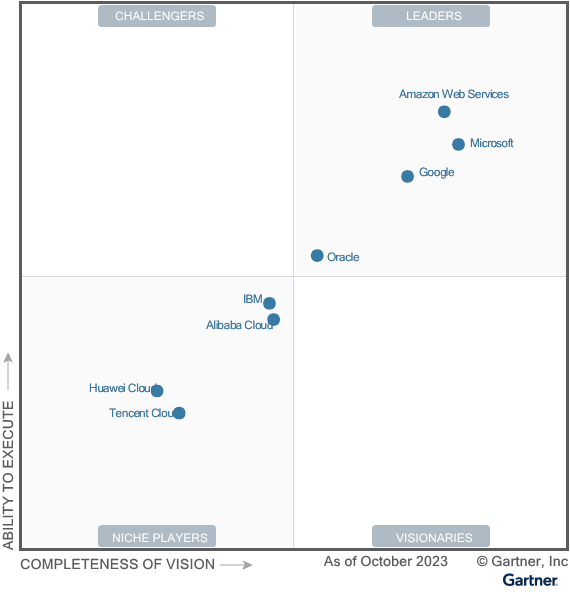
\includegraphics[width=0.8\textwidth]{gartner.png}
	\caption{Cuadrante mágico de Gartner para proveedores de nube}
	\label{fig:gartner}
\end{figure}

El resto de proveedores de nube, como \textit{IBM Cloud}, \textit{Oracle Cloud}
o \textit{Alibaba Cloud}, no se consideran en este estudio por su menor cuota de
mercado y su menor presencia en la industria.

\newpage{}
A continuación, se describen brevemente las características de cada uno de los
tres proveedores de nube considerados:

\begin{itemize}
	\item \textbf{Amazon Web Services (AWS)} es el proveedor de nube más grande y
		popular del mundo, con una amplia gama de servicios y herramientas que
		permiten a las empresas construir, desplegar y escalar aplicaciones en
		la nube de forma rápida y eficiente. AWS ofrece una infraestructura
		global con centros de datos en todo el mundo, lo que garantiza una alta
		disponibilidad y rendimiento de los servicios. Además, AWS cuenta con
		una amplia comunidad de usuarios y desarrolladores, lo que facilita la
		integración y el soporte de las aplicaciones en la nube.
	\item \textbf{Microsoft Azure} es otro proveedor de nube líder en el mercado
		conocido por su integración con las herramientas y servicios de
		Microsoft. El hecho de formar parte de las soluciones de Microsoft puede
		ser una ventaja para las empresas que ya utilizan sus productos, gracias
		a su integración con flujos de \textit{Office 365}, como es el caso de
		la Universidad de Oviedo.
	\item \textbf{Google Cloud Platform (GCP)} es el proveedor de nube de Google
		y, al igual que AWS y Azure, ofrece una amplia gama de servicios y
		herramientas para construir, desplegar y escalar aplicaciones en la nube.
		GCP es conocido por su enfoque en la innovación y la tecnología de
		vanguardia, lo que puede ser atractivo para empresas que buscan
		soluciones avanzadas y de alto rendimiento. Sin embargo, es la opción
		menos utilizada de las tres y ha tenido escándalos recientes de
		preservación de la información.\footnote{\href
			{https://www.business-standard.com/world-news/google-cloud-accidentally-deletes-125-billion-australian-pension-fund-124051800606_1.html}
			{Google Cloud accidentally deletes \$1.25 billion Australian pension fund}
		}
\end{itemize}

Pese a que las tres alternativas son válidas y ofrecen una amplia gama de
servicios y herramientas, la empresa ya utiliza la nube de Amazon para todas sus
aplicaciones y servicios, por lo que es la opción más lógica y coherente para
este proyecto. Además, AWS cuenta con servicios específicos referentes a
\textit{contenedores} que facilitarán el despliegue de la infraestructura y la
gestión de los servicios en la nube.


\newpage{}
\subsection{Sistemas de virtualización y servicios}\label{subsec:alt_servicios}
Okticket y el equipo de desarrollo utiliza \textit{Amazon Web Services} (AWS)
como proveedor de nube preferido para desplegar sus servicios y aplicaciones.
AWS ofrece una amplia gama de servicios y herramientas que permiten a las
empresas construir, desplegar y escalar aplicaciones en la nube de forma rápida
y eficiente. Dentro de la plataforma de AWS, existen varios tipos de
virtualización que pueden ser utilizados para implementar las funcionalidades
requeridas por el proyecto.

\paragraph{Amazon EC2} es el servicio de computación tradicional de AWS, que
permite lanzar máquinas virtuales con arquitecturas comunes de manera rápida.
Al tratarse de un sistema normal de máquinas virtuales, EC2 requiere el
mantenimiento de la máquina subyacente y la configuración e instalación del
motor de contenedores si se desea utilizar este tipo de tecnologías.

\paragraph{Amazon ECS} es un servicio de orquestación de contenedores que
permite ejecutar y escalar contenedores de Docker en la nube de AWS. ECS está
preparado para usar con Docker y proporciona una interfaz sencilla para
gestionar contenedores en entornos de producción. Sin embargo, ECS puede ser
complicado de configurar y gestionar, especialmente en entornos de gran escala.

\paragraph{Amazon EKS} es un servicio de orquestación de contenedores basado
en Kubernetes que permite ejecutar y escalar contenedores en la nube. EKS
proporciona una interfaz sencilla para gestionar clústeres de Kubernetes en
entornos de producción. EKS es una opción
popular para empresas que ya utilizan Kubernetes y desean aprovechar las
ventajas de la nube de AWS. Sin embargo, esto supondría plantear todo el
desarrollo desde cero en Kubernetes, un sistema que no se ha utilizado en la
empresa hasta la fecha y que requeriría una curva de aprendizaje significativa.

Para este proyecto, se decide utilizar \textit{Amazon ECS} como servicio de
orquestación de contenedores, ya que es una opción más sencilla y rápida de
desplegar que EKS y proporciona una interfaz intuitiva para gestionar
contenedores en la nube de AWS. ECS está diseñado para trabajar con Docker y
proporciona una solución completa para el despliegue y la gestión de
contenedores en entornos de producción, lo que facilitará el desarrollo y la
implementación de los servicios del sistema.


\newpage{}
\subsection{Tipos de máquinas}\label{subsec:alt_maquinas}
Una vez seleccionado el proveedor de nube y el servicio de orquestación, en
este caso \textit{Amazon ECS}, existen dos tipos de máquinas virtuales que se
pueden utilizar para desplegar los contenedores: \textit{EC2} y \textit{Fargate}.

\paragraph{Amazon EC2}, como ya se ha comentado, es el servicio de computación
tradicional de AWS que permite lanzar máquinas virtuales con arquitecturas
comunes de manera rápida. Al escoger esta opción, se tendría que gestionar el
\textit{tipo de instancia}\footnote{\url{
	https://aws.amazon.com/es/ec2/instance-types/
}} y la \textit{capacidad} de las máquinas, lo que puede acarrear más tiempo de
análisis y configuración.

\begin{figure}[H]
	\centering
	
\includegraphics[width=0.1\textwidth]{logos/ec2.png}
	\caption{Logo de Amazon EC2~\textregistered}
	\label{fig:ec2}
\end{figure}

\paragraph{AWS Fargate}\footnote{\url{https://aws.amazon.com/es/fargate/}} es un
servicio de contenedores de AWS con un enfoque más moderno que EC2, ya que
permite ejecutar contenedores sin necesidad de gestionar las máquinas
subyacentes. Fargate se encarga de aprovisionar y escalar la infraestructura
necesaria para ejecutar los contenedores en base a los recursos definidos en la
configuración. Aunque Fargate es más sencillo de usar y configurar que EC2,
también puede ser más costoso y menos flexible, ya que no es posible acceder
directamente a las máquinas subyacentes de manera sencilla o personalizar la
configuración de las instancias.

\begin{figure}[H]
	\centering
	
\includegraphics[width=0.1\textwidth]{logos/fargate.png}
	\caption{Logo de AWS Fargate~\textregistered}
	\label{fig:fargate}
\end{figure}

\paragraph{Decisión}
Dado que el proyecto no requiere una configuración específica de las máquinas
subyacentes y se busca una solución sencilla y rápida de desplegar, se decide
utilizar \textit{AWS Fargate} como servicio de contenedores para ejecutar los
servicios del sistema. Fargate provee una capa de abstracción sobre la
arquitectura subyacente, permitiendo centrarse el desarrollo de las
aplicaciones sin tener que preocuparse por más gestiones.
